%% ============================================================
%% SECTION*: Part I — Module-Wise Architectural Description
%% ============================================================

\section*{Part I: Module-Wise Architectural Description}

\subsection{Dense Inception Residual Convolution (DRIC) Blocks}

The first step in improving the classical U-Net architecture is to replace the $3\times3\times3$ convolution with something more modern that can capture both fine and coarse features in a single go. To address this limitation, inception-style parallel convolutions are employed, where parallel convolutional operations are performed using multiple sizes of kernels to extract feature on every scale. In our approach, we also added Dense and Residual Connections in the block so that feature preservation is improved during deep feature transformation. So, the fundamental feature extraction unit in our architecture combines three design principles: inception-style multi-branch convolution, dense connectivity, and residual learning, shown in Figure \ref{FIG:DRIC Block}.

\begin{center}
\begin{minipage}{\columnwidth}
    \centering

    % Main Figure
    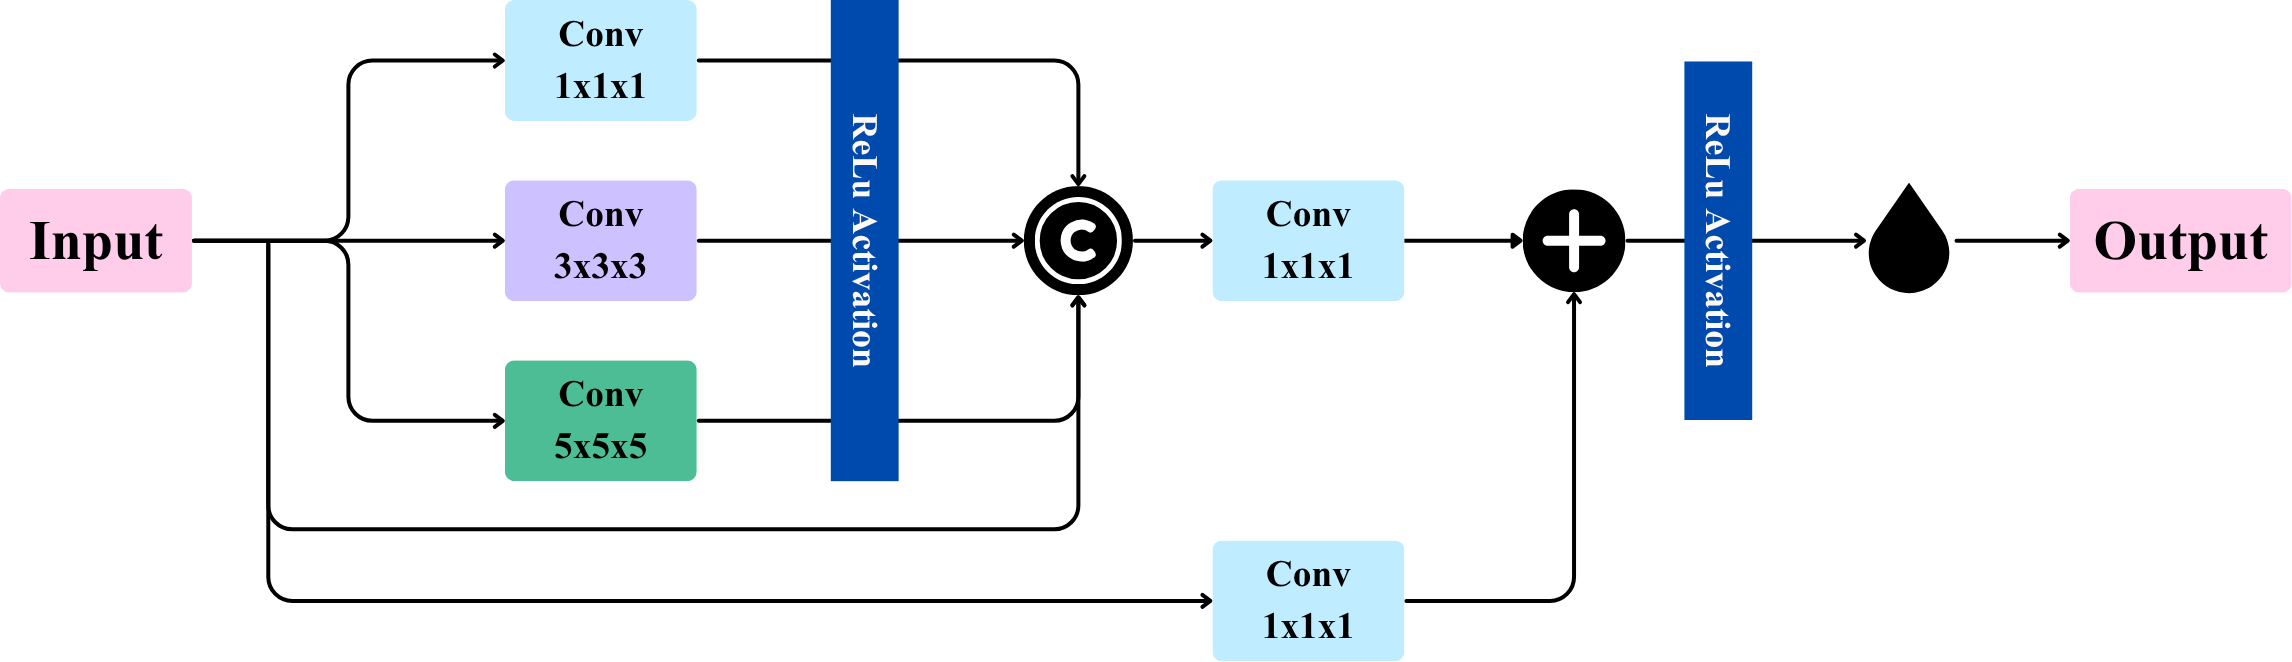
\includegraphics[
        height=0.085\textheight,
        width=0.9\textwidth
    ]{figs/Dense Inception-Residual Block.png}

    \vspace{1mm}

    % Dashed line settings
    \setlength{\dashlinedash}{0.5pt}
    \setlength{\dashlinegap}{1.5pt}

    % Legend Box
    \fbox{
    \begin{tabular}{cl|cl|cl}

    
\includegraphics[width=0.018\textwidth]{figs/Label1/1.png}
    &
    \hspace{-1.3em}
    \scriptsize Concatenation

    &

    
\includegraphics[width=0.018\textwidth]{figs/Label1/6.png}
    &
    \hspace{-1.3em}
    \scriptsize Dropout

    &

    
\includegraphics[width=0.018\textwidth]{figs/Label1/5.png}
    &
    \hspace{-1.3em}
    \scriptsize Add

    \\

    \end{tabular}
    }

    \captionof{figure}{Dense Inception-Residual Block}
    \label{FIG:DRIC Block}
\end{minipage}
\end{center}

\subsubsection{Inception-style multi-branch convolution}

Traditional convolutional layers use a single kernel size, which limits the receptive field per layer. Instead, the DRIC block applies multiple convolutional kernels of different sizes in parallel to capture features at different spatial scales. Formally, let the input tensor for the block be: $X\in H \times W \times D \times C_{in}$, where $H, W, D$ denote spatial dimensions, and $C_{in}$ is the number of input channels. Each branch applies a convolution with kernel size $\kappa\in 1,3,5:$
$F_k = \sigma(\mathcal W_k * X + b_k ), k\in 1,3,5,$ where * denotes 3D convolution, $\mathcal W_k$ and $b_k$ are trainable weights and biases, and $\sigma(\cdot)$ is a non-linear activation function (ReLU in our implementation).
The multi-branch outputs are concatenated channel-wise: $F_{concat} =[F_1 \| F_3 \| F_5 ],$ yielding a feature tensor enriched with both local fine details ($1\times 1\times 1$ and $3\times 3\times 3$) and broader contextual information ($5\times 5\times 5$).

\subsubsection{Dense connectivity}

To encourage feature reuse and strengthen gradient flow, the DRIC block incorporates dense connections. Instead of passing only the output of the previous block, the concatenation includes the input feature maps: $F_{dense} =[X \| F_{concat}]$. This ensures that each layer has direct access to all preceding feature maps, reducing redundancy, and improving parameter efficiency.

\subsubsection{Residual learning}

Direct stacking of inception-dense modules may increase feature dimensionality excessively, leading to optimization difficulties. To address this, the DRIC block applies a residual connection to stabilize training. A $1\times 1\times 1$ convolution is used to match the dimensions between the input and output before addition: $F_{res} =\sigma (\mathcal W_{res} * X + b_{res})$. Finally, the output of the DRIC block is: $Y = F_{dense} +F_{res}$. This residual formulation mitigates vanishing gradients and accelerates convergence by allowing the block to learn perturbations over the identity mapping rather than the full transformation.

\subsection{Multi-Scale Input Strategy}

\begin{center}
    \centering

    % Main Figure
    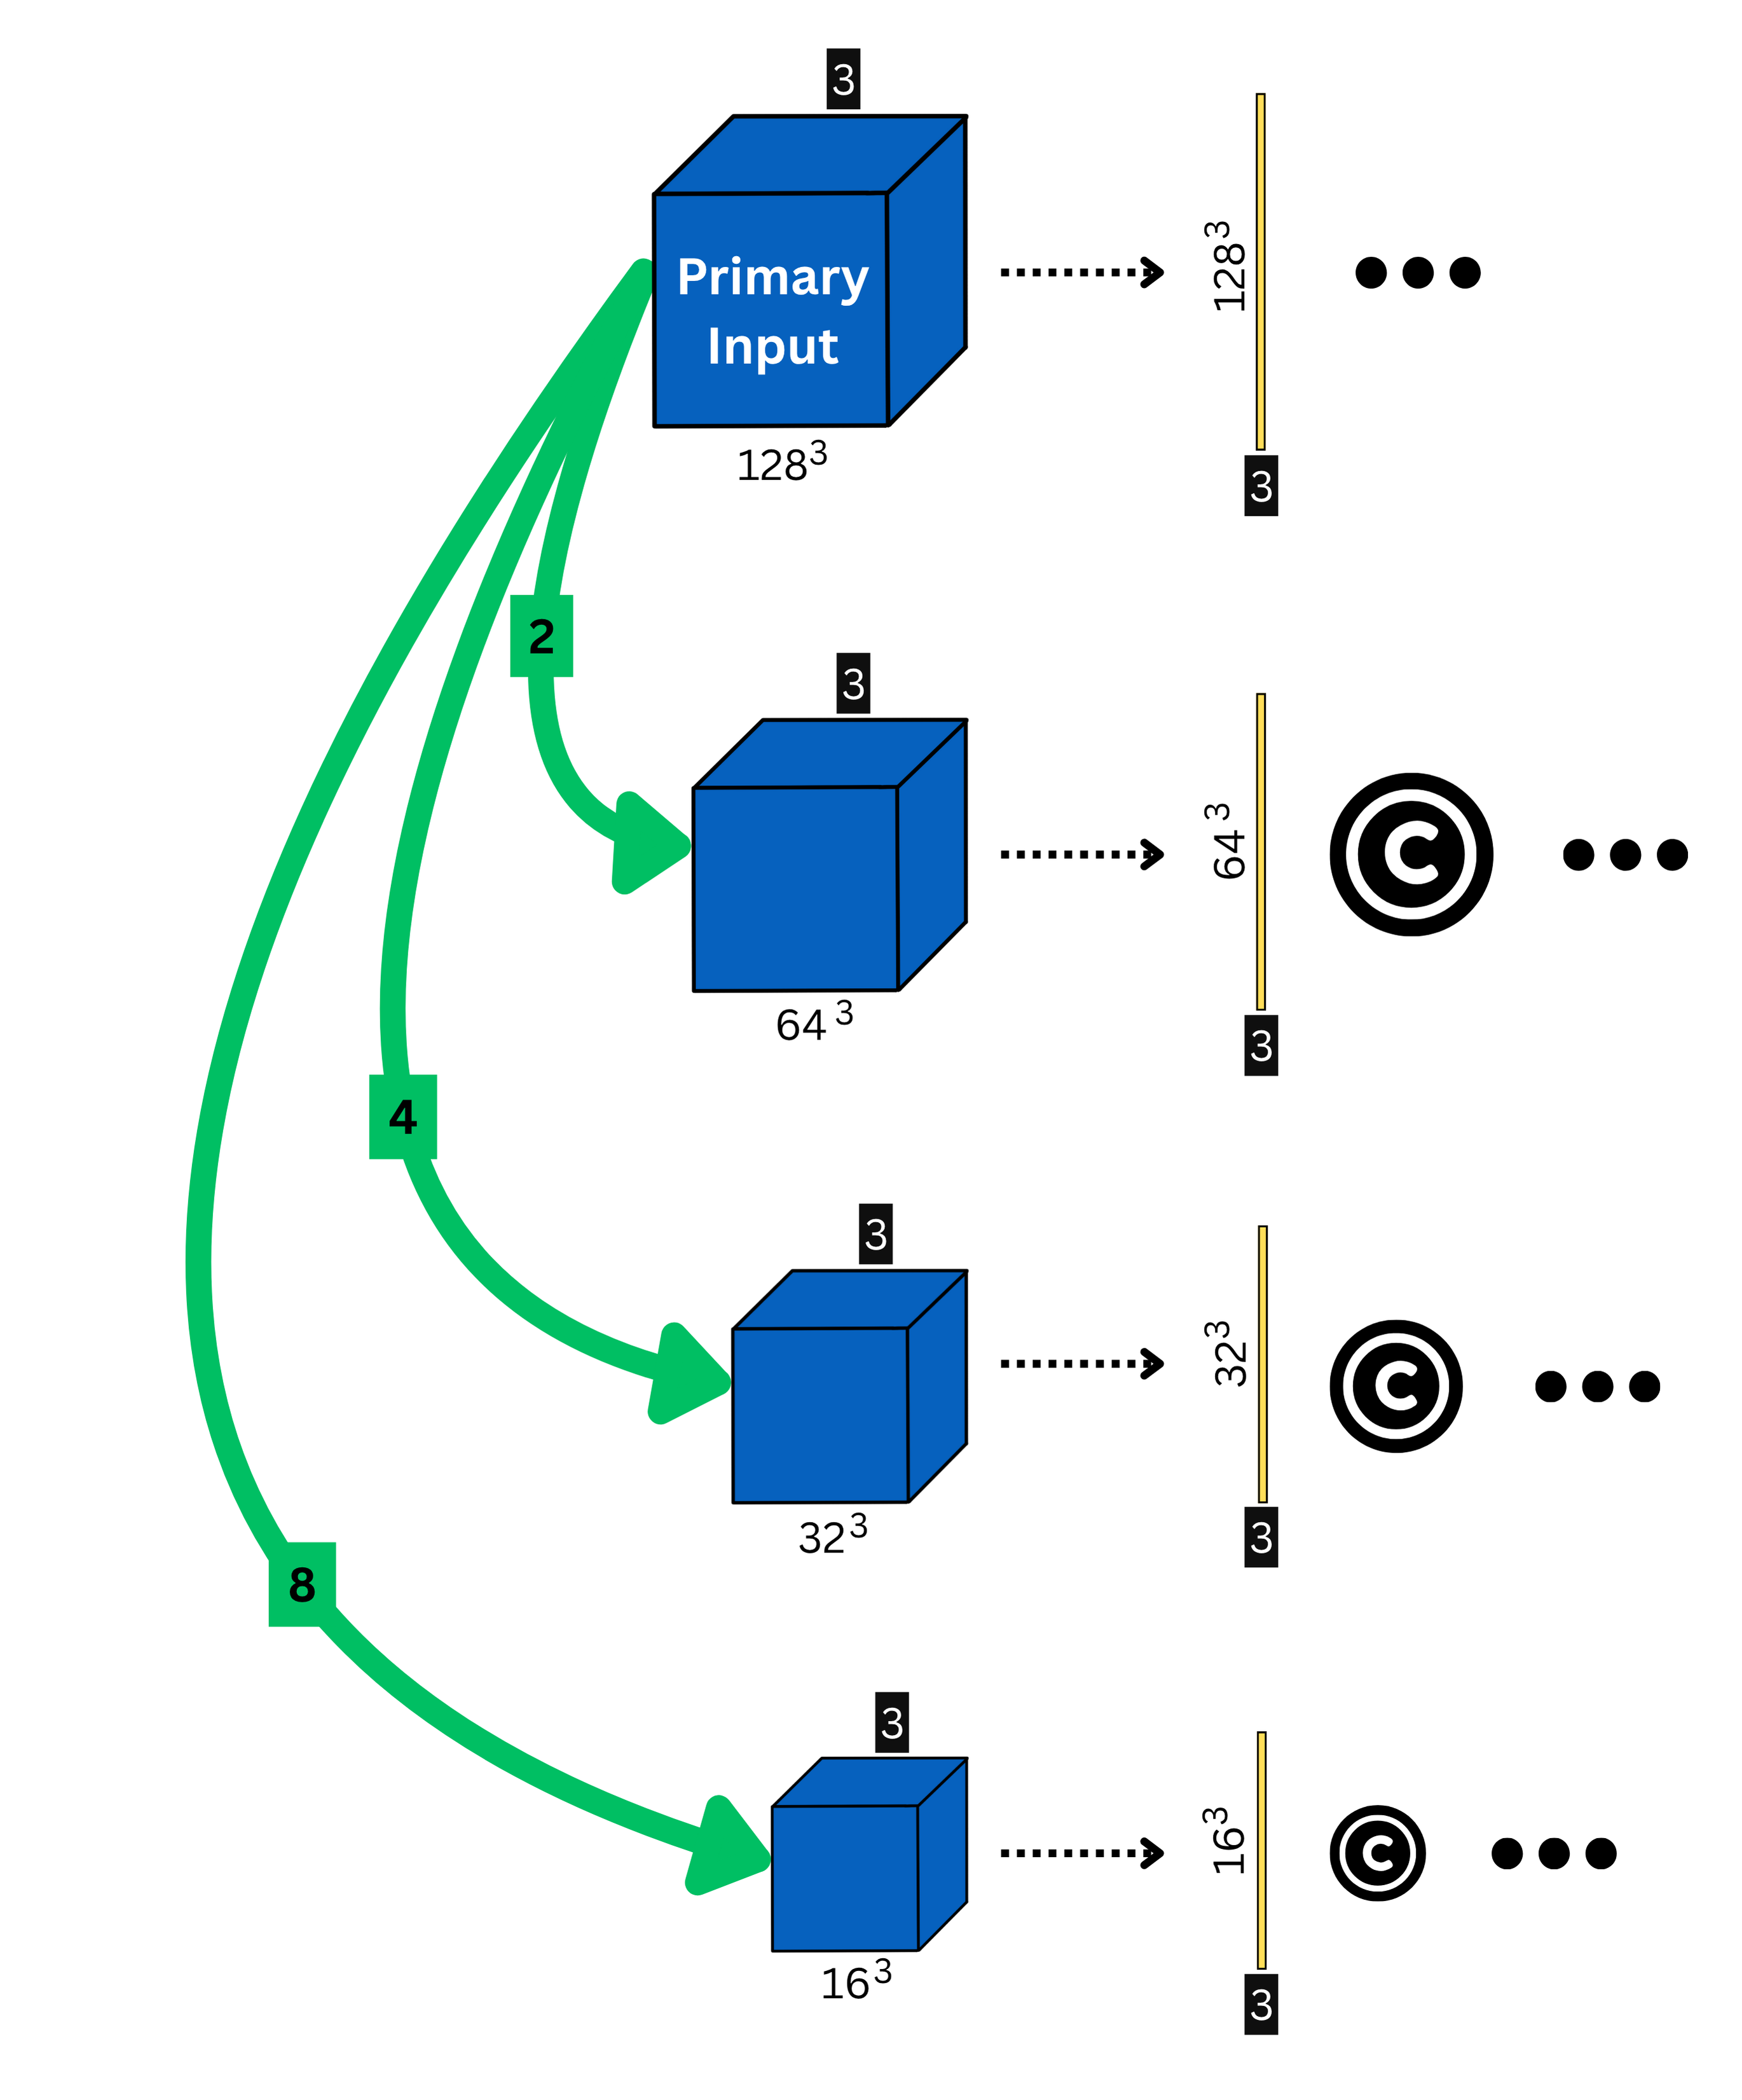
\includegraphics[
        %height=0.22\textheight,
        width=0.3\textwidth
    ]{figs/Input, Multi-Scale Paths.png}

    \vspace{2mm}

    % Dashed line settings
    \setlength{\dashlinedash}{0.5pt}
    \setlength{\dashlinegap}{1.5pt}

    % Legend Box
    \fbox{
    \begin{tabular}{cl|cl}

    
\includegraphics[width=0.018\textwidth]{figs/Label1/1.png}
    &
    \scriptsize Concatenation

    &

    
\includegraphics[width=0.032\textwidth]{figs/Label1/2.png}
    &
    \scriptsize Average-pooled by factor of $n$

    \\[1.5mm]

    \hdashline

    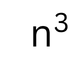
\includegraphics[width=0.030\textwidth]{figs/Label1/3.png}
    &
    \scriptsize Dimension

    &

    
\includegraphics[width=0.030\textwidth]{figs/Label1/4.png}
    &
    \scriptsize Number of channels

    \\

    \end{tabular}
    }

    \captionof{figure}{Multi-Scale Input Strategy}
    \label{FIG:Multi-Scale Input}

\end{center}

To enhance contextual understanding of tumors with highly variable size and appearance, our network incorporates a multi-scale input strategy shown in Figure \ref{FIG:Multi-Scale Input}. Instead of relying only on the hierarchical down-sampling of the encoder, we explicitly inject down-sampled versions of the input volume into the corresponding encoder stages.
Let the input be $X_0\in \mathbb{R}^{(128\times 128\times 128\times C)}, C=3,$ where $C$ is the number of MRI modalities (T1ce, T2, FLAIR). Scaled versions are obtained by applying a down-sampling operator $S_\kappa (\cdot): X_0^{(i)}=S_{2^{(i-1)}}(X_0), i=1,\cdots, 4,$ producing inputs at resolutions $128^3, 64^3, 32^3,$ and $16^3$. Each $X_0^{(i)}$ is passed through a shallow convolutional stem to produce features $F_0^{(i)},$ that are concatenated with encoder features $F_{l} $ at the corresponding stage $Z_{l} =Concat(F_{l} ,F_0^{(i)})$.
This design ensures that fine-scale structures ($e_\cdot g_\cdot$ enhancing tumor cores) are reinforced by high-resolution features, while large-scale abnormalities ($e_\cdot g_\cdot$ edema) benefit from the coarse global context. Empirically, the multi-scale input improved boundary precision and reduced false positives compared to encoder-only baselines.


\subsection{Encoder (Contracting Path)}

\begin{center}
    \centering

    % Main Figure
    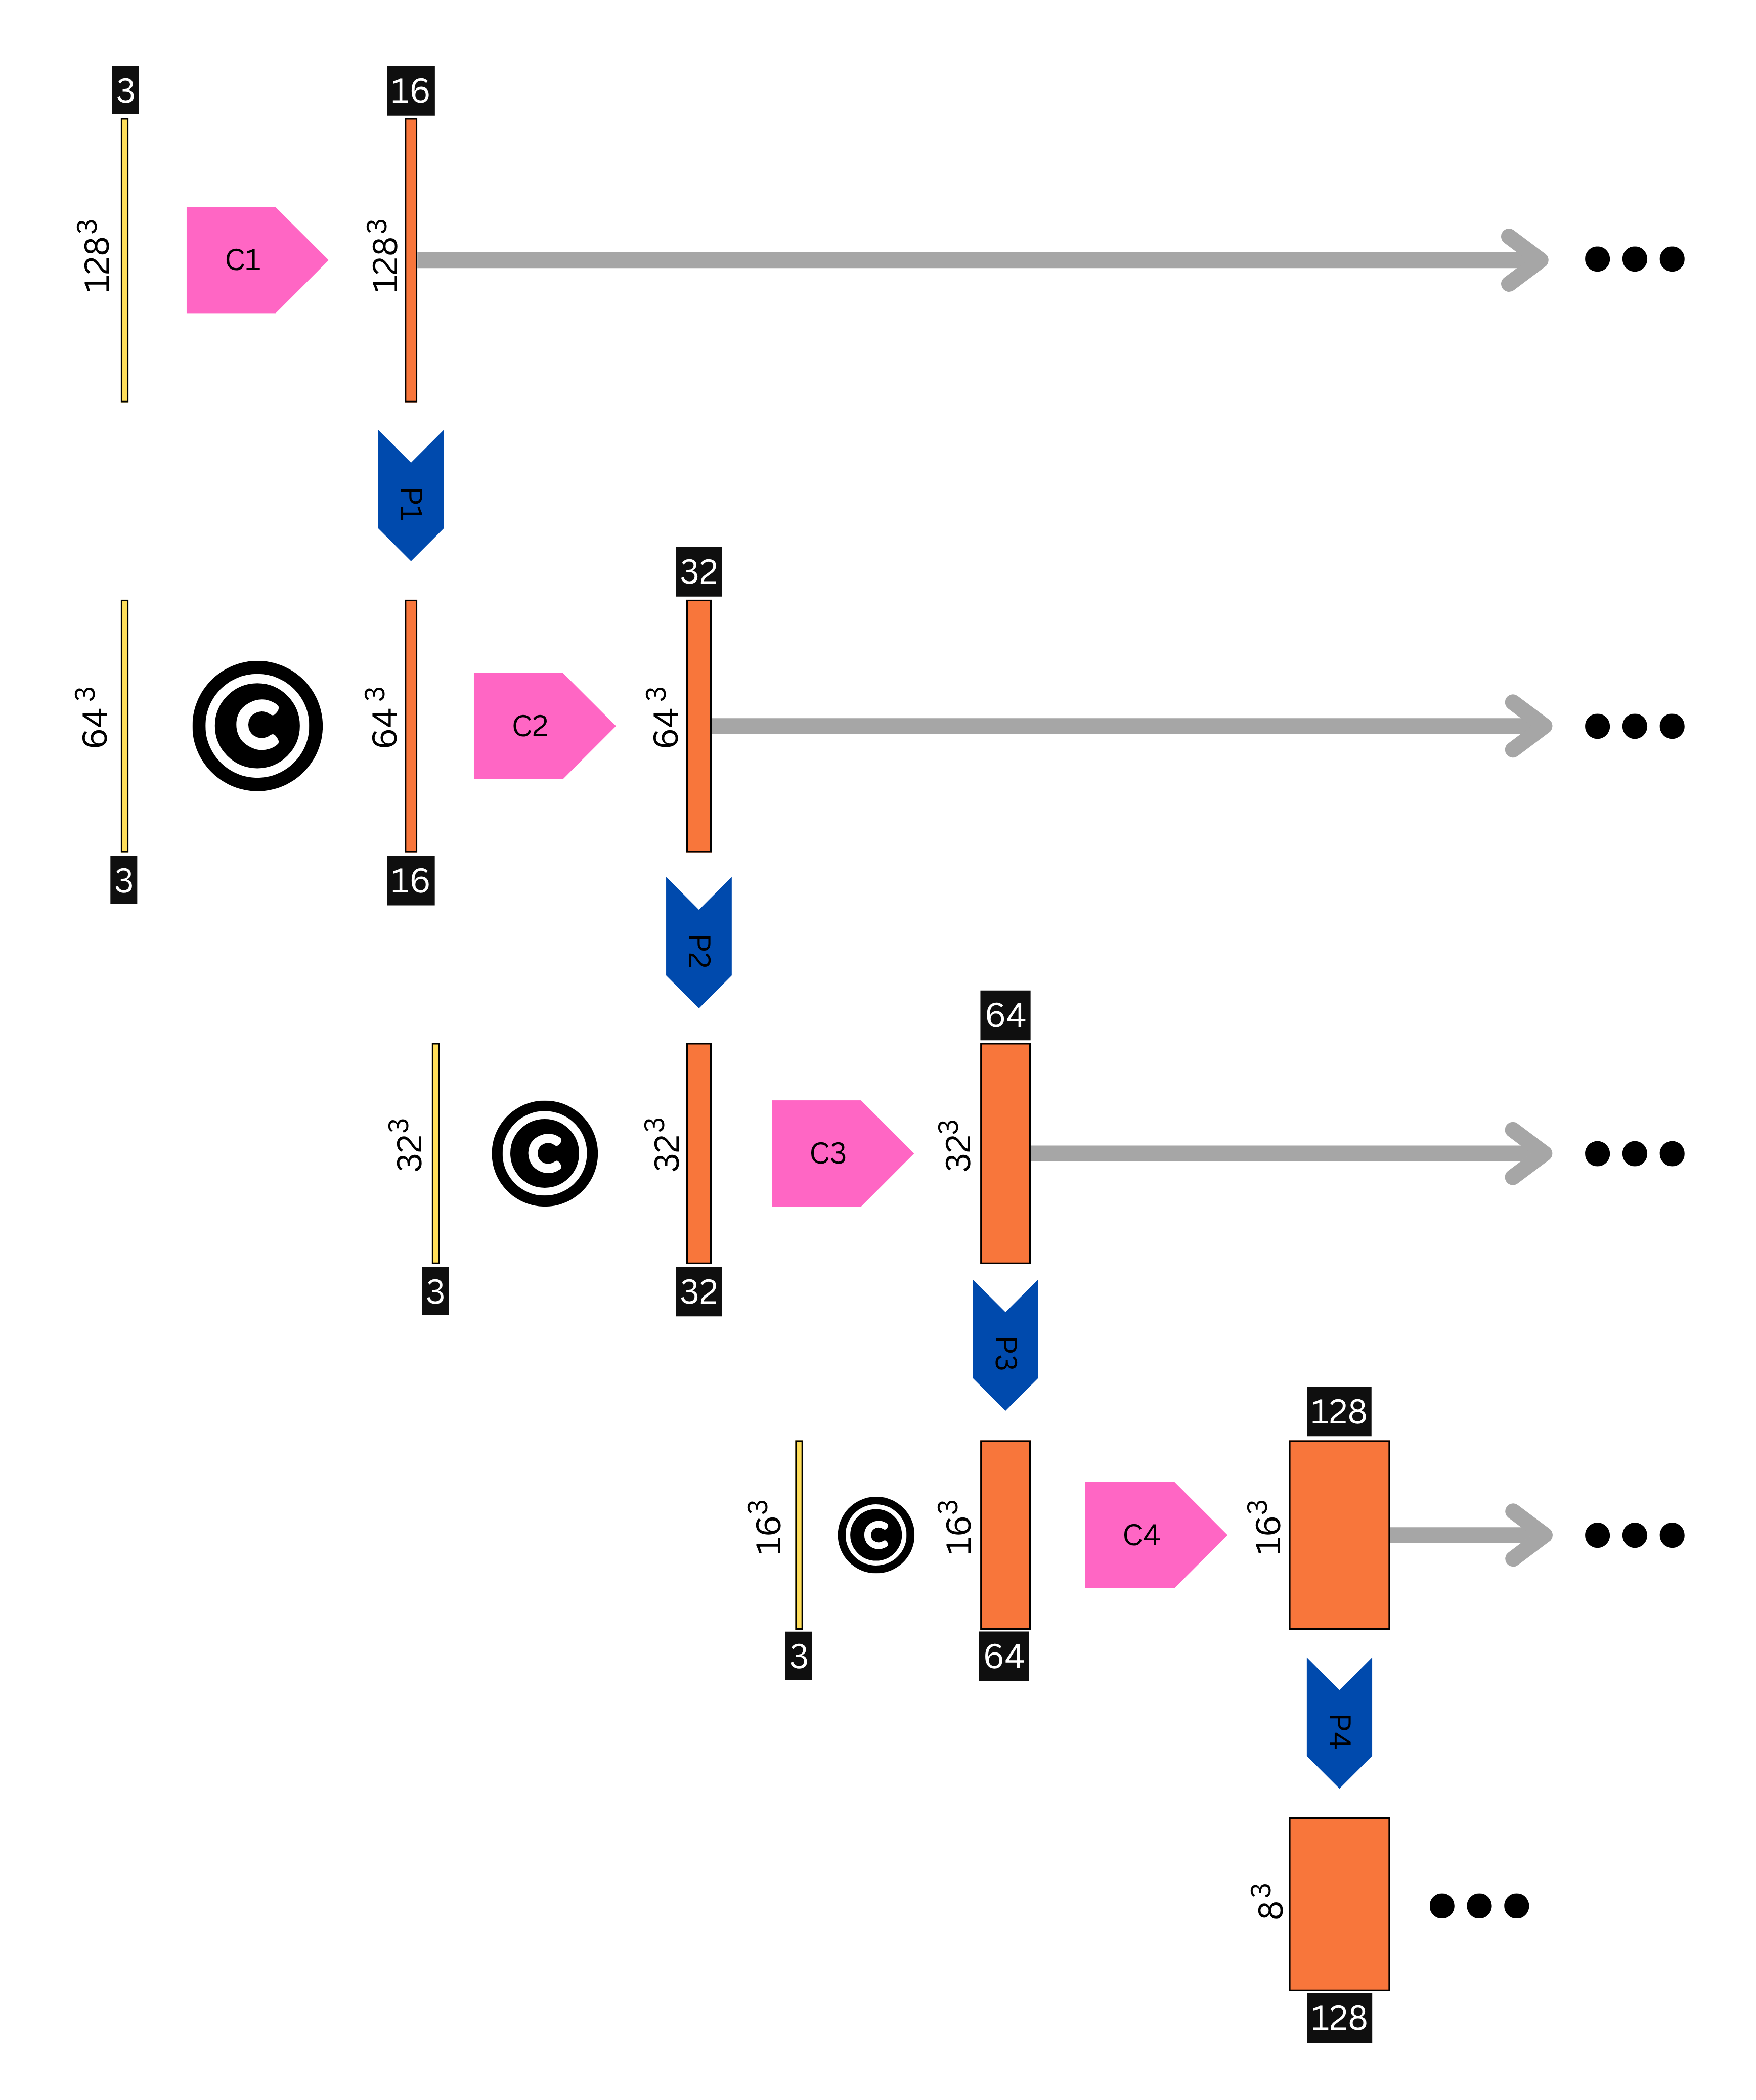
\includegraphics[
        %height=0.22\textheight,
        width=0.3\textwidth
    ]{figs/Encoder Path.png}

    \vspace{2mm}

    % Dashed line settings
    \setlength{\dashlinedash}{0.5pt}
    \setlength{\dashlinegap}{1.5pt}

    % Legend Box
    \fbox{
    \begin{tabular}{cl|cl}

    
\includegraphics[width=0.018\textwidth]{figs/Label1/1.png}
    &
    \scriptsize Concatenation

    &

    
\includegraphics[width=0.015\textwidth]{figs/Label1/9.png}
    &
    \scriptsize MaxPool

    \\[1.5mm]

    \hdashline

    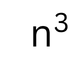
\includegraphics[width=0.030\textwidth]{figs/Label1/3.png}
    &
    \scriptsize Dimension

    &

    
\includegraphics[width=0.030\textwidth]{figs/Label1/4.png}
    &
    \scriptsize Number of channels

     \\[1.5mm]

    \hdashline

    
\includegraphics[width=0.030\textwidth]{figs/Label1/8.png}
    &
    \scriptsize Dense Inception-Res Block

    \\

    \end{tabular}
    }

    \captionof{figure}{Encoder Path}
    \label{FIG:Contracting Path}

\end{center}

The encoder path, in Figure \ref{FIG:Contracting Path}, of our network is designed to progressively down-sample the input volume while simultaneously extracting rich hierarchical features. This is achieved by stacking multiple DRIC blocks interleaved with down-sampling operations (3D max-pooling).
Let the network input be: $X\in \mathbb{R}^{(H\times W\times D\times C_0)},$ where in our implementation the spatial dimensions are $128\times 128\times 128$ with $C_0 = 3$ representing the number of input channels, namely T1ce, T2 and FLAIR. Applying a DRIC block to each encoder stage $l$, the transformation corresponds to: $F_l=DRIC_l(X_{l-1}),$ where $X_{l-1}$ is the input to stage $l$, and $F_l$ is the output feature tensor. Extending the prior definition of the DRIC block $F_l$ can be expressed as $F_l=[X_{l-1} \| \sigma(W_1 *X_{l-1}) \| \sigma(W_3 *X_{l-1} ) \| \sigma(W_5 *X_{l-1} )]+W_{res} *X_{l-1}$, where $1, 3,$ and $5$ represent the kernel sizes in the inception-style parallel branches, while the final summation corresponds to the residual mapping.
After feature extraction, spatial resolution is reduced by applying 3D max pooling with stride 2:   $X_l=MaxPool3D(F_{l,p=2}),$ where $p$ is the size of pooling window. This leads to a twofold reduction in spatial dimensions: $H_l=\tfrac{H_{l-1}}{2}, W_l=\tfrac{W_{l-1}}{2}, D_l=\tfrac{D_{l-1}}{2}$. Thus, the encoder creates progressively deeper representations while shrinking the spatial extent.
The encoder is composed of L-stages, each consisting of one DRIC block followed by down-sampling. In practice, $L=4$. The recursive formulation is: $X_l=MaxPool3D(DRIC_l (X_{l-1})), l=1,\cdots,L$.
At the end of the encoder, we obtain a multi-resolution feature pyramid: $F=\{F_1,F_2,\cdots,F_L\},$ where $F_l$ represents features at stage $l$ before pooling. These tensors are later forwarded to the decoder through skip connections.


\subsection{Decoder (Expanding Path)}

\begin{center}
    \centering

    % Main Figure
    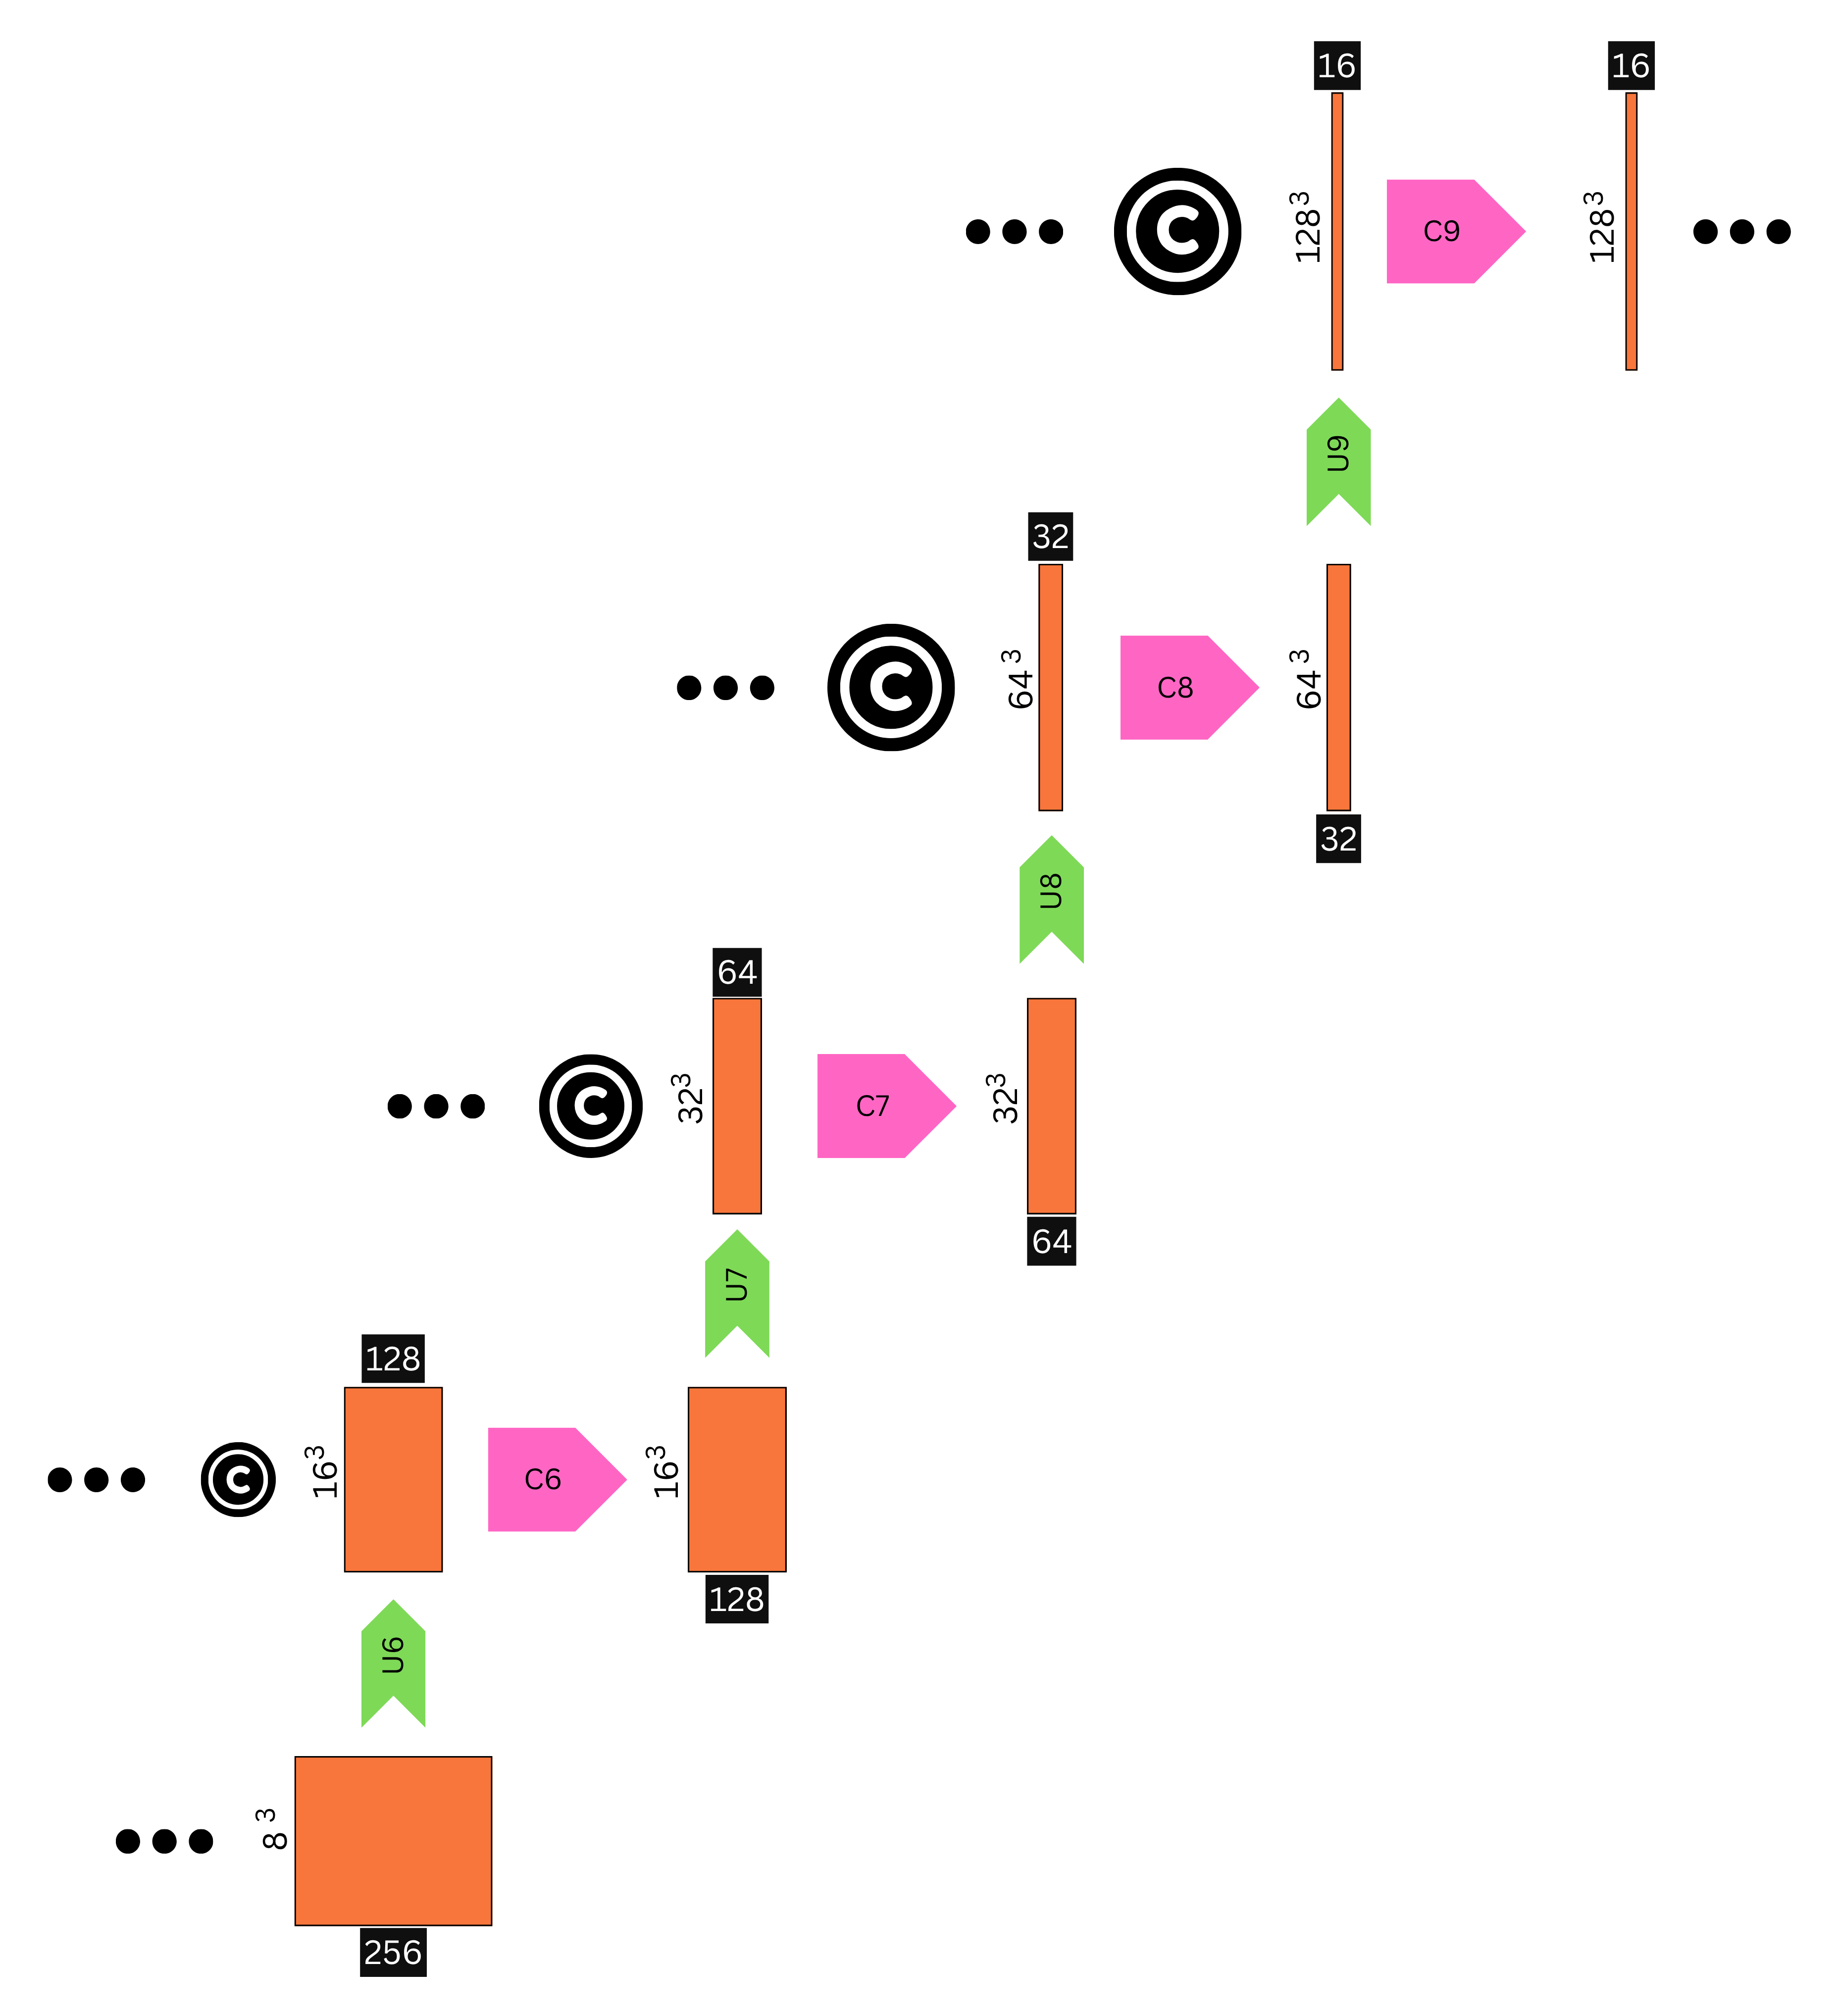
\includegraphics[
        height=0.22\textheight,
        width=0.33\textwidth
    ]{figs/Decoder Path.png}

    \vspace{2mm}

    % Dashed line settings
    \setlength{\dashlinedash}{0.5pt}
    \setlength{\dashlinegap}{1.5pt}

    % Legend Box
    \fbox{
    \begin{tabular}{cl|cl}

    
\includegraphics[width=0.018\textwidth]{figs/Label1/1.png}
    &
    \scriptsize Concatenation

    &

    
\includegraphics[width=0.015\textwidth]{figs/Label1/7.png}
    &
    \scriptsize TransConv

    \\[1.5mm]

    \hdashline

    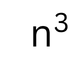
\includegraphics[width=0.030\textwidth]{figs/Label1/3.png}
    &
    \scriptsize Dimension

    &

    
\includegraphics[width=0.030\textwidth]{figs/Label1/4.png}
    &
    \scriptsize Number of channels

     \\[1.5mm]

    \hdashline

    
\includegraphics[width=0.030\textwidth]{figs/Label1/8.png}
    &
    \scriptsize Dense Inception-Res Block

    \\

    \end{tabular}
    }

    \captionof{figure}{Decoder Path}
    \label{FIG:Expanding Path}

\end{center}

The decoder path, in Figure \ref{FIG:Expanding Path}, of our network is designed to progressively up-sample the compressed bottleneck representation and reconstruct the segmentation mask at full resolution. This is achieved by combining learned up sampling operators, attention-gated skip connections, and DRIC blocks for feature refinement.
Let the bottleneck feature map be: $X\in \mathbb{R}^{(H_B\times W_B\times D_B\times C_B)}, where H_B, W_B, D_B$ are the spatial dimensions of the bottleneck and $C_B$ the number of channels. The decoder consists of $L$ stages that mirror the depth of the encoder.
At each decoder stage $l$, the first operation is learned up-sampling by a 3D transposed convolution: $U_l=ConvTranspose3D(X_{l+1},k=2,s=2),$ where $k$ is the kernel size and s the stride. This doubles the spatial dimensions: $H_l=2H_{l-1}, W_l=2W_{l-1}, D_l=2D_{l-1}$.
The up sampled tensor $U_l$ is then fused with the encoder feature map $F_l$ via an attention gate. The gating function suppresses irrelevant encoder activations and is defined as: $S_l=\alpha_l\odot F_l, \alpha_l=\sigma(W_u U_l+W_e F_l+b),$ where $\sigma$ is the sigmoid function, $W_u, W_e$ are learnable projections and $\odot $ is element-wise multiplication. This ensures that only the salient encoder features are propagated.
The decoder feature at stage $l$ is then formed by concatenating the up-sampled tensor and the attended skip features: $C_l= U_l \| S_l$ followed by calling the DRIC block to integrate multi-scale convolutions and residual mappings as $F_l^{'}= DRIC_l (C_l)$.
The recursive formulation of the decoder is thus: {\footnotesize$X_l= DRIC_l (Concat(ConvTranspose3D(X_{l+1}),A(F_l,X_{l+1}))), l = L,\cdots,1,$} where $A(\cdot)$ denotes the attention gate.
At the final stage, the reconstructed feature map has the same resolution as the input volume. A $1\times 1\times 1$ convolution followed by a voxel-wise softmax projects it to class probabilities: $\hat{Y} = Softmax(W_0 * X_1 + b_0), \hat{Y} \in \mathbb{R}^{H\times W\times D\times K},$ where $K$ is the number of segmentation classes. Each voxel $(i,j,k)$ is assigned a label by: $\hat{y}_{(i,j,k)} = \arg\max \hat{Y}^{(c)}_{(i,j,k)}$.
Thus, the decoder path progressively restores spatial detail while leveraging both encoder information (via attention-gated skip connections) and multi-scale feature extraction (via DRIC refinement).


\subsection{Skip Connections, Attention Gates and Bottlenecks}

\begin{center}
    \centering
    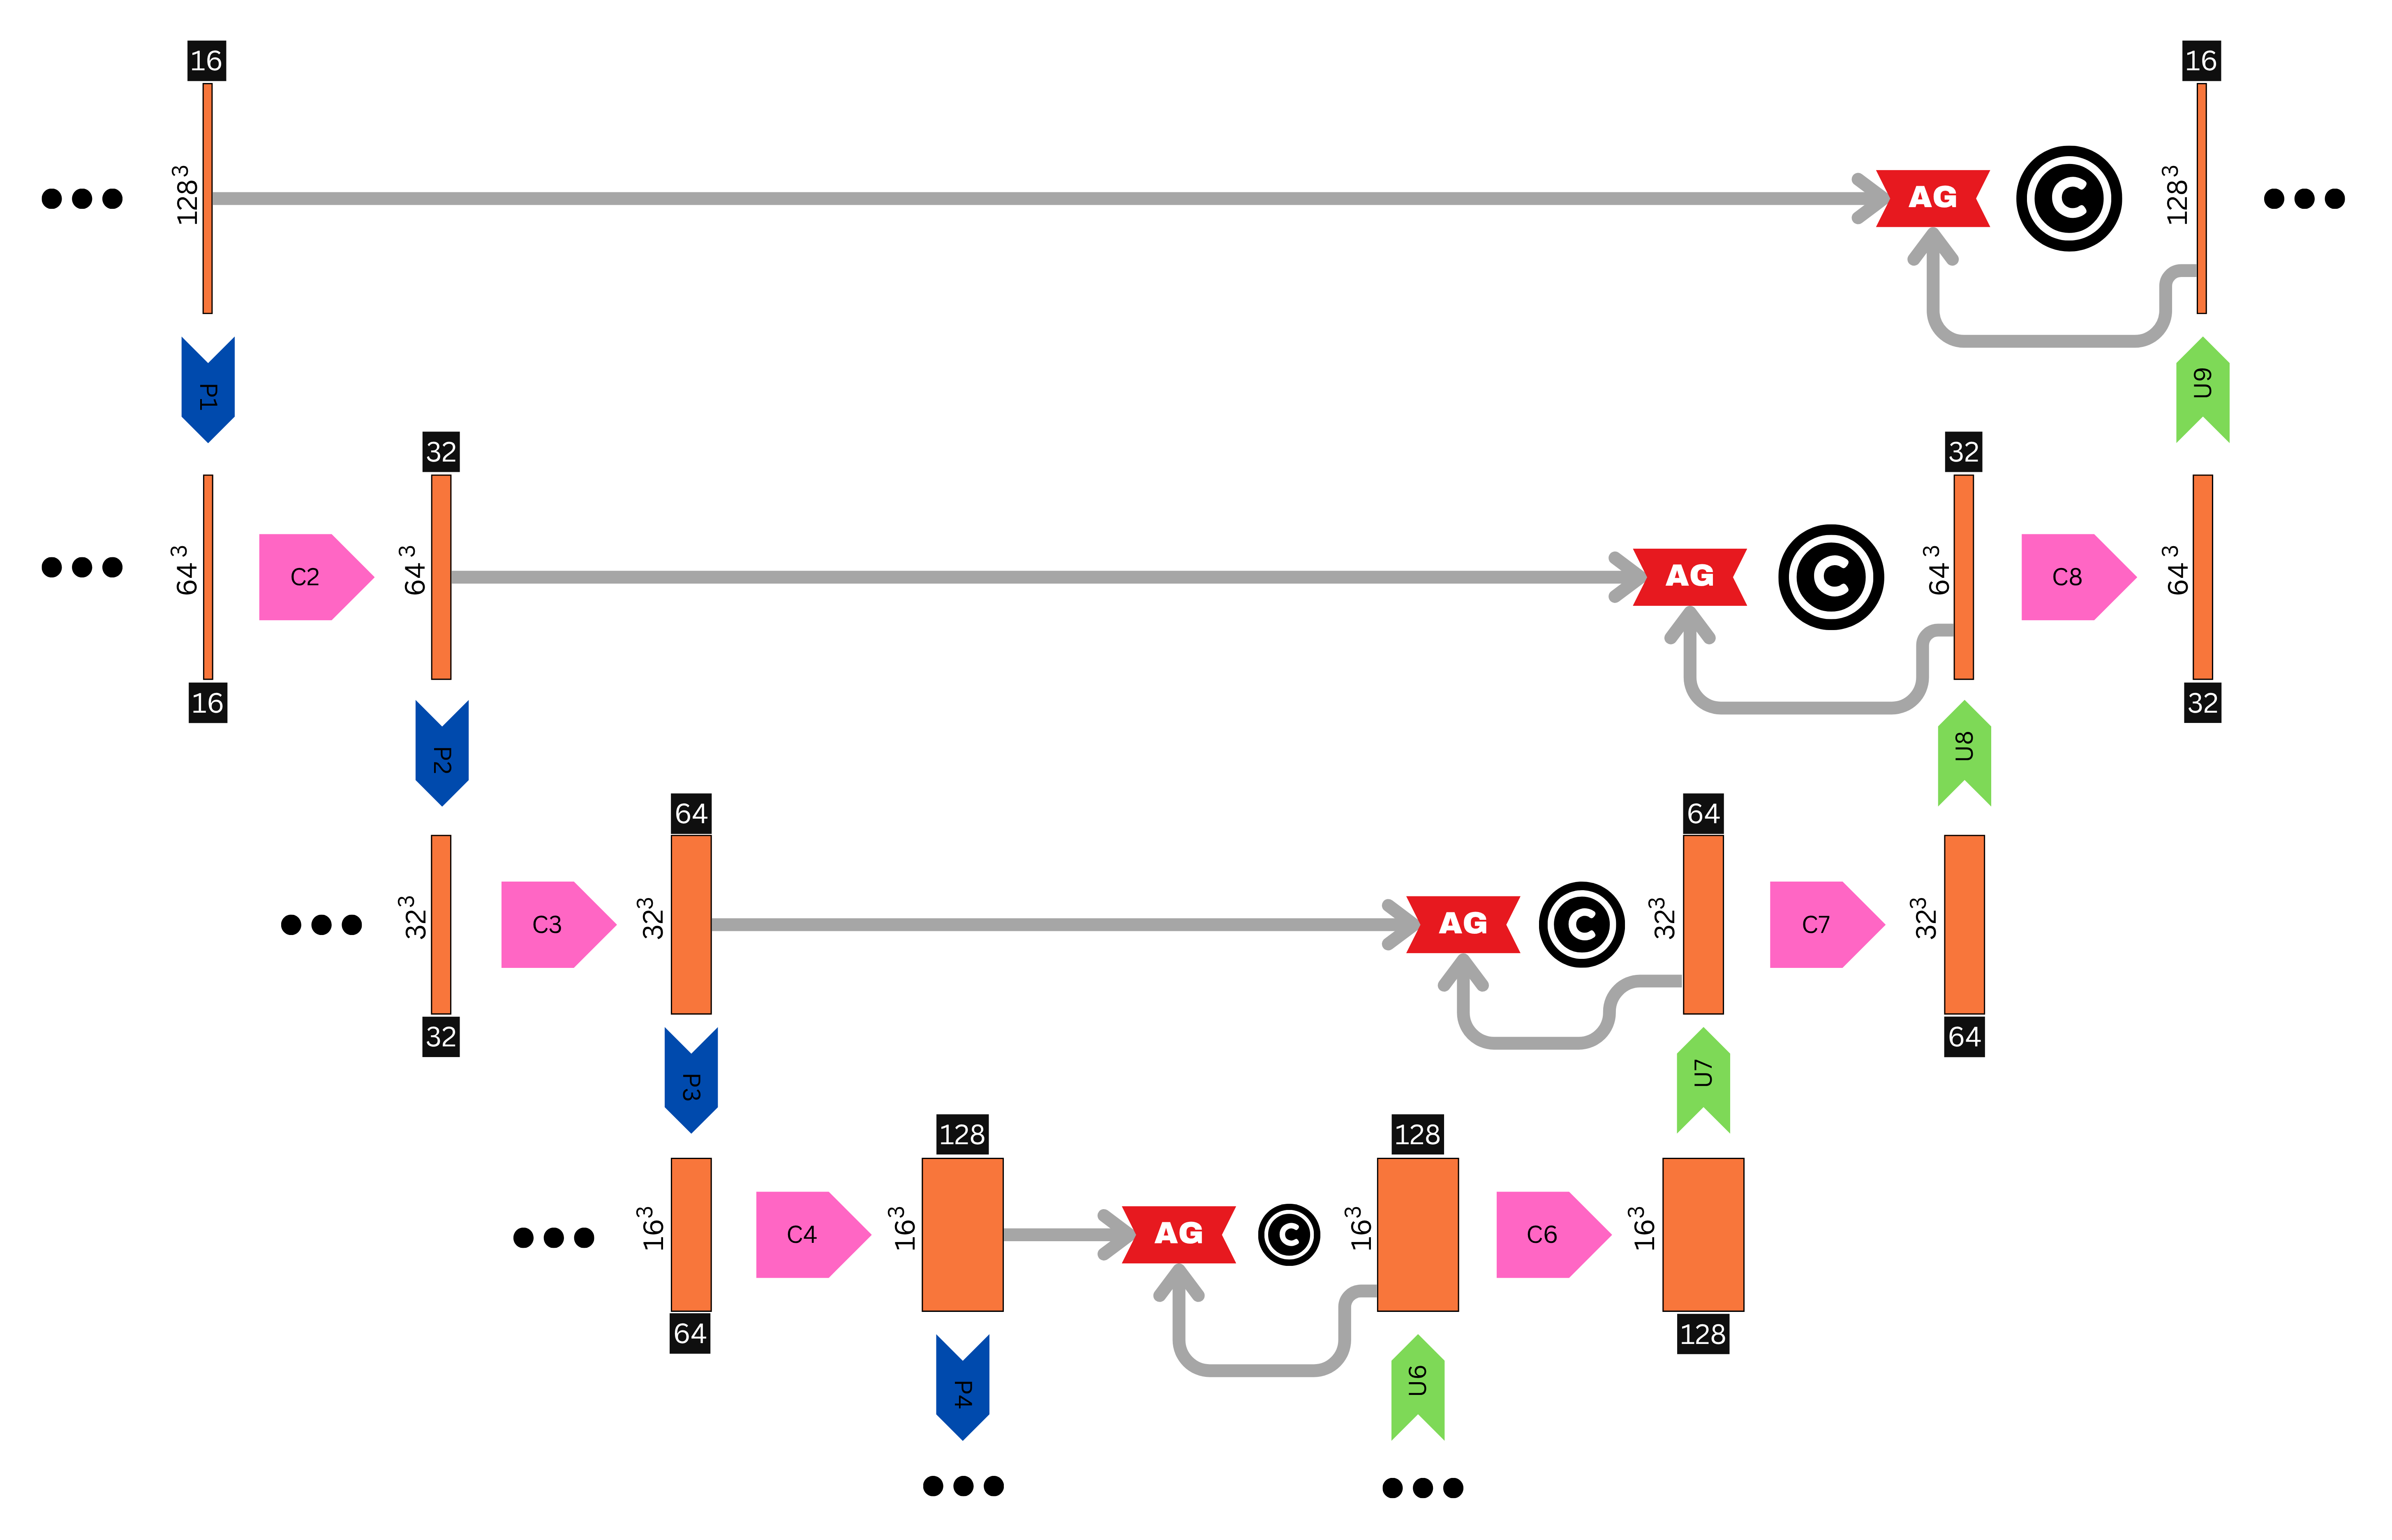
\includegraphics[height=0.17\textheight, width=0.4\textwidth]{figs/Attention gates over skip connections.png}

    \vspace{2mm}

    % Dashed line settings
    \setlength{\dashlinedash}{0.5pt}
    \setlength{\dashlinegap}{1.5pt}

    % Legend Box
    \fbox{
    \begin{tabular}{cl|cl}

    
\includegraphics[width=0.018\textwidth]{figs/Label1/1.png}
    &
    \scriptsize Concatenation

    &

    
\includegraphics[width=0.015\textwidth]{figs/Label1/9.png}
    &
    \scriptsize MaxPool

    \\[1.5mm]

    \hdashline

    
\includegraphics[width=0.015\textwidth]{figs/Label1/7.png}
    &
    \scriptsize TransConv

    &

    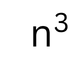
\includegraphics[width=0.030\textwidth]{figs/Label1/3.png}
    &
    \scriptsize Dimension

    \\[1.5mm]

    \hdashline

    
\includegraphics[width=0.030\textwidth]{figs/Label1/4.png}
    &
    \scriptsize Number of channels

    &

    
\includegraphics[width=0.030\textwidth]{figs/Label1/8.png}
    &
    \scriptsize Dense Inception-Res Block

    \\[1.5mm]

    \hdashline

    
\includegraphics[width=0.030\textwidth]{figs/Label1/10.png}
    &
    \scriptsize AttentionGate

    \\

    \end{tabular}
    }

    \captionof{figure}{Skip Connections, Attention Gates and Bottleneck}
    \label{FIG:Attention gates over skip connections}
\end{center}

The skip connections in our architecture, in Figure \ref{FIG:Attention gates over skip connections}, follow the classical U-Net design principle, in which feature maps from the encoder stages are directly forwarded to their corresponding decoder stages. This mechanism ensures that high-resolution spatial features suppressed by down-sampling are preserved and reintegrated during up-sampling, thereby enhancing localization accuracy. Formally, let $F_l\in \mathbb{R}^{H_l\times W_l\times D_l\times C_l}$ denote the feature map at encoder stage $l$; the skip connection then transmits $F_l$ to the decoder stage with the corresponding resolution.
However, instead of transmitting the encoder features unfiltered, our model incorporates Attention Gates (AGs) to refine the skip connections. These gates are designed to suppress irrelevant activations (e.g., healthy tissue) while amplifying responses from salient tumor regions. Mathematically, each gate computes an attention coefficient for every spatial position $(i,j,k)$ in the feature tensor, based on both the encoder feature $F_l$ and a gating signal $G$ from deeper layers: $\alpha =\sigma (W_\alpha^T (\psi_F * F_l + \psi_G * G + b)),$ where * denotes convolution, $\psi_F$ and $\psi_G$ are learnable transformations of the encoder and gating signals, respectively, and $\sigma(\cdot)$ is the sigmoid activation ensuring values between 0 and 1. The attended feature map is then given by: $\Tilde{F}_l = \alpha \odot F_l,$ where $\odot$ denotes element-wise multiplication. This selective mechanism allows the network to dynamically highlight tumor-relevant regions while reducing background noise.
At the bottleneck stage, the network processes the lowest-resolution feature map, where the receptive field is maximized, and semantic abstraction is strongest. The bottleneck consists of stacked DRIC blocks operating on $F_L$ , the deepest encoder feature, thereby enabling multi-scale contextual aggregation before the decoder begins reconstruction. Unlike the encoder or decoder stages, no pooling or up-sampling is applied here; instead, the bottleneck provides a dense representation that captures global tumor context across the entire 3D patch.
